% ------------------------------------------------------------------------
% file `1_E_juin-transferer-23-exercise-body.tex'
%   in folder `xsim/'
%
%     exercise of type `transferer' with id `23'
%
% generated by the `transferer' environment of the
%   `xsim' package v0.21 (2022/02/12)
% from source `1_E_juin' on 2023/06/06 on line 474
% ------------------------------------------------------------------------
    Dans le cadre d’une exposition, un artiste a empilé des canettes. L’illustration ci-dessous montre les trois rangées du haut du montage.
    \begin{multicols*}{2}
        \begin{center}
            \begin{tblr}{
                    hlines,
                    vlines,
                    columns={3cm, c},
                    rows={1cm,m},
                    row{1}={gray!40, font=\bfseries},
                }
                Numéro de la rangée & Nombre de canettes par rangées \\
                1                   & 1                              \\
                2                   & 4                              \\
                3                   & 7                              \\
                4                   &                                \\
                5                   &                                \\
                6                   & 16                             \\
            \end{tblr}
        \end{center}

        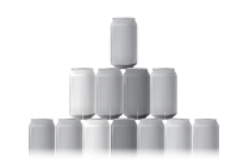
\includegraphics{img/cannettes.png}
    \end{multicols*}

    \begin{enumerate}
        \item Complète le tableau.
        \item Détermine le nombre de canettes de la 9ème rangée.
        \item Détermine le nnuméro de la rangée qui comporte 31 canettes.
        \item Propose une formule qui permet de calculer le nombre de canettes \(c\) nécessaire en fonction du numéro de la rangée \(n\). \\
              \(c=\)
    \end{enumerate}
